\documentclass[journal]{IEEEtran}

\usepackage{amsmath,amssymb,amsfonts}
\usepackage{graphicx}
\usepackage{booktabs}
\usepackage{cite}
\usepackage{algorithm}
\usepackage{algorithmic}

\newcommand{\E}{\mathbb{E}}
\newcommand{\Prb}{\Pr}
\newcommand{\median}{\mathrm{median}}
\newcommand{\R}{\mathbb{R}}
\newcommand{\Cset}{\mathcal{C}}
\newcommand{\N}{\mathcal{N}}

\author{\IEEEauthorblockN{Zhiguo Xiao\textsuperscript{1,2,*},
Yujing Guo\textsuperscript{2}, Yanqi Shao\textsuperscript{2},
Guangteng Chen\textsuperscript{2}, Dingbo Hou\textsuperscript{2},
Yuanyuan Liu\textsuperscript{2}, Xinyao Cao\textsuperscript{1,2}, Junli Liu\textsuperscript{1,2}}
\IEEEauthorblockA{\textsuperscript{1}School of Computer Science and Technology,
Beijing Institute of Technology, Beijing 100081, China\\
\textsuperscript{2}School of Computer Science and Technology,
Changchun University, Changchun 130022, China}
\IEEEauthorblockA{\textsuperscript{*}Corresponding author: Zhiguo Xiao
(email: 3220215169@bit.edu.cn)}}

\title{Budget-Aware Event-Level Rate-Normalized Early Warning for Bearings in Industrial IoT: Validation in a Virtual IoT Environment}

\markboth{IEEE Internet of Things Journal}%
{Xiao \MakeLowercase{\textit{et al.}}: Budget-Aware Event-Level Rate-Normalized Early Warning}

\begin{document}
\maketitle

\begin{abstract}
Predictive maintenance in the Industrial Internet of Things requires joint control of edge detection, event delivery, and fleet-scale false-event budgets. This paper proposes budget-aware event-level rate-normalized detection (BA-RNED). A node converts nonnegative RMS excess above an early-life baseline into a time-averaged excess rate and latches the first alarm at a frozen threshold; a gateway deduplicates and retries compact events; a fleet layer converts a false-event budget into a calibration-quantile requirement. On IMS, XJTU-SY, and FEMTO/PRONOSTIA, RNED detects 31/34 failures (exact 95\% CI: 76.3--98.1\%) with median leads of 14.5\%, 46.3\%, and 36.0\% of life; five healthy-evidence tiers show that it is not inherently alarm-free. A D1-causal-three ablation shows that public D1's 33/34 advantage depends on endpoint confirmation: without it, detection is 34/34 but healthy-censored alarms are 8/8. On Jetson Orin NX, an update costs 0.03235~ms and 0.0383~mJ. In a 100-machine simulation, event traffic saves 98.043\% bytes without loss, and one retry under 10\% loss achieves 98.999\% delivery. BA-RNED contributes a reproducible causal event protocol and budget boundary rather than a more complex diagnostic model.
\end{abstract}

\begin{IEEEkeywords}
Industrial IoT, bearing prognostics, edge computing, early warning, event budgeting, virtual IoT, false alarms.
\end{IEEEkeywords}

\section{Introduction}\label{sec:intro}
Predictive maintenance in industrial IoT must output a latchable, transmittable, and budgetable first maintenance event rather than a sequence of sample-level anomaly scores; machinery-health and deep-learning surveys frame the broader data-to-decision pipeline~\cite{lei2018,fink2020}. Sensor nodes continuously acquire vibration, but raw-waveform uploading consumes bandwidth and energy. If the cloud receives continuous scores, it must still choose an alarm threshold, confirmation rule, and fleet-level tolerance. Treating every deviation as a fault causes unnecessary shutdowns, whereas confirming a state only at the endpoint removes the online value of a warning.

The research gap is the absence of a failure-versus-drift discriminator that, under a zero-false-alarm constraint, simultaneously supports causal updating, a fixed threshold, interpretability, edge deployment, lead-time reporting, and fleet-event accounting. Accordingly, this paper examines four questions: (1) which trajectory statistic separates failure-bound degradation from benign drift under healthy-censored controls; (2) whether that statistic yields a causal, fixed-threshold detector with $O(1)$ state updates; (3) whether rate normalization is necessary and effective relative to classical, deep-reconstruction, and supervised-RUL baselines; and (4) whether edge cost, quantization robustness, and fleet-event capacity satisfy IIoT deployment constraints.

The central idea is to convert ``how far above baseline is the amplitude'' into ``what is the average nonnegative excess during monitoring.'' For each axis, RMS snapshots define an early-life median baseline $b$; the relative amplitude is $r_t=f_t/b$ and the nonnegative excess is $e_t=\max(r_t-1.2,0)$. Failure-bound excess tends to occur more often and with larger magnitude, whereas benign transients are diluted by the monitoring duration. A single causal threshold therefore tests accumulated excess load rather than instantaneous amplitude.

The main contributions are as follows. First, we propose the rate-normalized RMS-excess detector and factor the time-averaged excess into exceedance frequency and positive-excess magnitude; full-life and fixed-window audits prevent persistence alone from being overinterpreted. Second, under one causal protocol and zero-false-alarm calibration, we compare classical detectors, the closest RMS-ratio rule, persistence rules, deep reconstruction models, and an RUL baseline, including leave-one-IMS-experiment-out sensitivity. Third, we measure edge latency and energy, add causal 8-bit feature quantization, deterministic byte accounting, and a modeled fleet-event budget, while making explicit that the study validates a node-side detector rather than a complete multi-node IIoT system.

The remainder is organized as follows. Section~\ref{sec:related} reviews related work. Section~\ref{sec:framework} presents BA-RNED. Section~\ref{sec:method} formalizes the detector. Section~\ref{sec:experiments} describes the experimental protocol. Section~\ref{sec:results} reports results. Section~\ref{sec:discussion} discusses mechanism, statistical boundaries, and engineering implications. Section~\ref{sec:conclusion} concludes.

\section{Related Work}\label{sec:related}
\subsection{Health indicators and early-warning rules}
RMS, kurtosis, skewness, and peak-to-peak amplitude have long been used for bearing monitoring~\cite{dyer1978}, while envelope analysis characterizes impulsive faults~\cite{randall2011}. Smith and Randall benchmarked common indicators on CWRU data~\cite{smith2015}, and reviews emphasize monotonicity, robustness, and early sensitivity~\cite{wangd2018}. These lightweight, causal indicators are suitable for edge nodes, but one snapshot cannot distinguish persistent degradation from transient drift. This work does not introduce a new index; it converts RMS excess into a time-averaged event rate.

Cross-condition fault diagnosis is related but different: transfer, domain-adaptation, and domain-generalization methods reduce training/deployment distribution mismatch~\cite{xiao2024dg}. They mainly identify fault categories, whereas this work uses each machine's early-life baseline for single-machine degradation warning.

\subsection{Classical online change detection}
Shewhart monitors the current sample~\cite{shewhart1931}, CUSUM accumulates positive deviations~\cite{page1954}, EWMA smooths exponentially~\cite{roberts1959}, and SPRT applies sequential likelihood ratios~\cite{wald1945}. These are the closest online baselines, but unbounded accumulators can be pushed upward by positive healthy excess under a fixed zero-false-alarm threshold. We quantify this failure under the same protocol and identify time normalization as the key difference.

\subsection{Unsupervised OOD and anomaly detection}
Deep one-class and confidence-based OOD methods learn a healthy or known-class distribution~\cite{ruff2018,hendrycks2017}; stochastic recurrent networks and TranAD represent time-series anomaly detection~\cite{su2019,tuli2022tranad}. These methods usually score sample- or window-level deviation and do not by themselves distinguish transient drift from persistent accumulated excess.

\subsection{Supervised RUL regression}
From early neural networks to attention-based models, RUL research has developed a rich literature~\cite{wang2020,gebraeel2004,chen2021}. These methods require degradation labels and predict remaining life. This work requires only a healthy baseline and outputs a maintenance event, so the RUL model is an advantage-mismatched comparison rather than an equivalent task.

\subsection{IoT edge intelligence}
Edge computing and TinyML support on-device processing under latency, bandwidth, and energy constraints~\cite{lu2023edge,abadade2023tinyml}; federated diagnosis and unsupervised IoT time-series learning further characterize large-scale systems~\cite{xiao2024bcefl,liu2023iot}. BA-RNED is a low-state first-event trigger for such systems, not a replacement for high-capacity diagnosis.

\subsection{Closest label-free warning protocol}
An unpublished protocol evaluated RMS-ratio rules on IMS and tested transfer across three datasets~\cite{hora_submitted,hora_unpublished}. We retain its early-life baseline and 1.2-fold excess idea, but distinguish a single-sample rule, endpoint-persistent D1, and the causal event rate under identical calibration.

\section{BA-RNED: Budget-Aware Event-Level Framework}\label{sec:framework}
BA-RNED extends the rate-normalized detector to a node--gateway--fleet protocol without changing the node's online state. The node computes RMS, calibrates an early-life baseline, updates a time-averaged excess rate, and latches one alarm. It stores only cumulative excess $S_t$ and monitoring count $t$.

The gateway receives an event ID, timestamp, triggering axis, score, and a compact diagnostic summary. The ID gives idempotent deduplication; data and ACK packets may be independently lost and retried. Raw waveforms are not forwarded.

Given fleet size $F$, tolerable expected false events $B$, and acceptable fleet probability $\alpha=B/F$, a per-machine false-event probability $q$ must satisfy
\begin{equation}
1-(1-q)^F\le\alpha,\qquad q\le1-(1-\alpha)^{1/F}.
\end{equation}
The point estimate is not used directly to choose a threshold. Instead, the fleet layer uses a conservative upper confidence quantile of the healthy calibration distribution; when the tail quantile cannot be estimated, it triggers secondary confirmation or human review rather than extrapolating zero false alarms from a small sample.

\section{System Model and Rate-Normalized Detector}\label{sec:method}

\subsection{Overview}
The three layers have distinct responsibilities: the mechanism layer tests whether excess persistence is discriminative, the statistical layer states the strength and assumptions of false-alarm control, and the engineering layer constrains state, computation, communication, and fleet-level alarm budget. This separation prevents a mechanism analogy, an empirical operating point, or an edge benchmark from being over-read as a universal guarantee.

The framework splits an offline discrimination stage and an online warning stage that share one feature chain and one discriminative signal. The input is the per-snapshot vibration feature of each bearing--axis stream (the online path uses RMS; the offline OOD benchmark uses RMS/kurtosis/skewness/variance/peak-to-peak); the output is a failure-versus-drift score (offline) and a latching alarm time (online). The modules run as: feature self-extraction $\to$ early-life baseline estimation $\to$ excess computation $\to$ time averaging (rate) $\to$ fixed-threshold alarming; the dataflow is strictly causal, and the score at any time depends only on current and past snapshots. The methodological stance is that RMS is not fault-specific and $e_i$ is not an estimate of physical damage; their value is a nonnegative, monotone, broadband energy-increment observable at sub-millisecond cost, making irreversible accumulation statistically separable from reversible drift. The novelty lies in two places: defining the discriminative signal as the \emph{cumulative excess} of RMS above a $1.2\times$ baseline (offline, the corresponding question), and rewriting that cumulative quantity in a \emph{rate-normalized} online form with a single fixed threshold (online, the corresponding question), compared against CUSUM/SPRT/Shewhart/EWMA and modern deep-reconstruction/RUL baselines under one protocol . Fig.~\ref{fig:arch} shows the overall architecture.

\begin{figure}[!t]
\centering
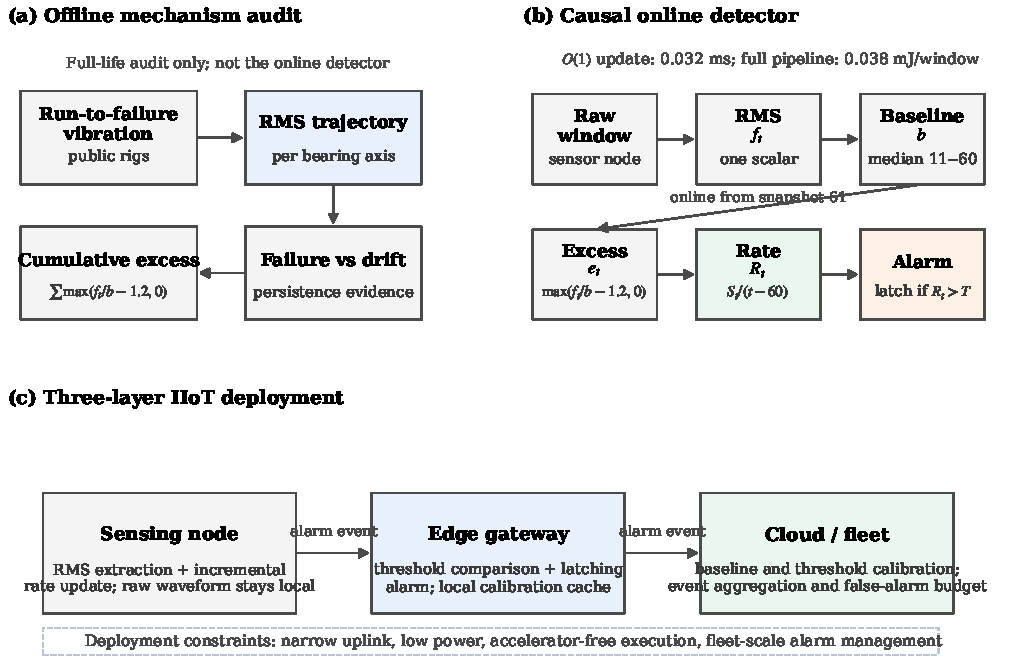
\includegraphics[width=\linewidth]{../figures/fig1_architecture.pdf}
\caption{Overall architecture: (a) the offline discrimination stage identifies the failure-versus-drift signal via the cumulative excess; (b) the online deployment stage is a causal six-step chain in which the RMS feature is baseline-calibrated and excess-rate--transformed before a single fixed threshold raises the alarm; (c) the three-layer IIoT deployment---sensing node (RMS + rate update), edge gateway (threshold + latching alarm), and cloud/fleet (batch calibration + aggregation)---with alarm-only uplink.}
\label{fig:arch}
\end{figure}

The middle panel of Fig.~\ref{fig:arch} collapses the online method into a six-step causal chain: raw vibration $\to$ RMS feature $f_i$ $\to$ baseline $b$ $\to$ excess rate $R_t$ $\to$ fixed threshold $T$ $\to$ latching alarm. Except for baseline estimation, every step is an incremental per-snapshot update that never accesses future data---the concrete meaning of ``causal and deployable.'' The right panel gives the three-layer IIoT deployment form (sensing node / edge gateway / cloud-fleet), developed in Section~\ref{sec:deploy}. The timeline also defines our lead-time convention: the alarm-to-failure interval as a percentage of life \eqref{eq:leadtime}, which avoids the incomparable cross-rig clocks (600\,s / 60\,s / 10\,s).


\subsection{Problem formalization and notation}
Consider one axis stream of one bearing. Let the $i$-th snapshot contain $m$ samples $x_{i,j}$ ($j=1,\dots,m$), with $N$ snapshots in total. The scalar health feature used by the online path is the per-snapshot RMS
\begin{equation}
f_i=\left(\frac{1}{m}\sum_{j=1}^{m}x_{i,j}^{2}\right)^{1/2}.
\label{eq:rms}
\end{equation}
The offline OOD benchmark additionally uses Pearson kurtosis, sample skewness, population variance, and peak-to-peak, computed from the same $x_{i,j}$ by their standard definitions and not numbered separately. The healthy baseline $b$ and relative amplitude $r_i$ are
\begin{equation}
b=\mathrm{median}\left\{f_i:11\le i\le60\right\},\qquad r_i=\frac{f_i}{b},
\label{eq:baseline}
\end{equation}
where the baseline window is snapshots 11--60 (discarding the first 10 run-in snapshots). The per-snapshot excess $e_i$ is the positive part of the relative amplitude above threshold $c$:
\begin{equation}
e_i=\max\left(r_i-c,\,0\right),\qquad c=1.2.
\label{eq:excess}
\end{equation}
Equations~\eqref{eq:rms}--\eqref{eq:excess} define the four basic quantities: $f_i$ the health feature, $b$ the healthy baseline, $r_i$ the normalized amplitude, and $e_i$ the per-snapshot excess. Table~\ref{tab:notation} collects all symbols.

\begin{table}[!t]
\caption{Notation used in this paper.}
\label{tab:notation}
\centering
\begin{tabular}{l l l}
\toprule
Symbol & Meaning & Type/range\\
\midrule
$x_{i,j}$ & $j$-th sample of the $i$-th snapshot & real\\
$m$ & samples per snapshot & positive integer\\
$f_i$ & RMS feature of the $i$-th snapshot \eqref{eq:rms} & nonnegative real\\
$i,t$ & snapshot index & positive integer\\
$N$ & total snapshots of the axis stream & positive integer\\
$b$ & early-life baseline \eqref{eq:baseline} & nonnegative real\\
$c$ & excess threshold (ratio), 1.2 & $c>1$\\
$r_i$ & relative amplitude \eqref{eq:baseline} & nonnegative real\\
$e_i$ & per-snapshot excess \eqref{eq:excess} & nonnegative real\\
$E_{\mathrm{cum}}$ & cumulative excess \eqref{eq:cumexcess} & nonnegative real\\
$S_t$ & excess running sum \eqref{eq:runningsum} & nonnegative real\\
$R_t$ & rate (time-averaged excess) \eqref{eq:rate} & nonnegative real\\
$T$ & alarm threshold (fixed scalar) \eqref{eq:threshold} & nonnegative real\\
$\tau$ & first alarm snapshot \eqref{eq:alarm} & $61,\dots,N$ or $\infty$\\
$L$ & lead time (\% of life) \eqref{eq:leadtime} & $0$--$100\%$\\
$\mathcal{C}$ & censored (healthy) bearing set & set\\
\bottomrule
\end{tabular}
\end{table}


\subsection{Offline discriminative feature: cumulative excess}\label{sec:cumexcess}
\emph{Motivation.} the corresponding question requires separating failure-bound degradation from benign drift under a zero-false-alarm constraint. The intuition is that the exceedances of a failed bearing accumulate persistently while benign drift is only occasional; integrating the ``part above $1.2\times$ baseline'' over the whole life decouples persistence from amplitude. \emph{Definition.} The cumulative excess is the whole-life sum of \eqref{eq:excess}:
\begin{equation}
E_{\mathrm{cum}}=\sum_{i=61}^{N}e_i=\sum_{i=61}^{N}\max\left(\frac{f_i}{b}-c,\,0\right).
\label{eq:cumexcess}
\end{equation}
Equation~\eqref{eq:cumexcess} (code identifier \texttt{auc\_above\_1p2x}) is a whole-life offline quantity that uses future snapshots and cannot be deployed online; it answers the corresponding question---on IMS the four failed and eight censored bearings are fully separated (AUROC 100, Section~\ref{sec:rq2})---and motivates the online form of Section~\ref{sec:rate}.


\subsection{Online rate-normalized detector}\label{sec:rate}
\emph{Motivation.} Turning the cumulative quantity into a time average makes the score independent of monitoring duration---the key to ``a single fixed threshold transfers across rigs,'' and the mechanism the corresponding question tests. For $O(1)$ memory and $O(1)$ time we use a running-sum recursion:
\begin{equation}
S_t=S_{t-1}+e_t,\qquad S_{60}=0.
\label{eq:runningsum}
\end{equation}
The rate (time-averaged excess) is
\begin{equation}
R_t=\frac{S_t}{t-60}=\frac{1}{t-60}\sum_{i=61}^{t}e_i,\qquad t\ge61.
\label{eq:rate}
\end{equation}
The \emph{alarm rule} is a latching first crossing:
\begin{equation}
\tau=\min\left\{t\ge90:R_t>T\right\};
\label{eq:alarm}
\end{equation}
if the set in \eqref{eq:alarm} is empty then $\tau=\infty$ (no alarm); $t\ge90$ means at least 30 monitored snapshots. The \emph{threshold calibration} (one-time, offline, censored set $\mathcal{C}$ only) is
\begin{equation}
T=1.01\cdot\max_{k\in\mathcal{C}}\max_{t\ge61}R_t^{(k)}.
\label{eq:threshold}
\end{equation}
The \emph{lead time} (percentage of life) is
\begin{equation}
L=\frac{N-\tau}{N-60}\times100\%.
\label{eq:leadtime}
\end{equation}
\emph{Length invariance (the mechanism behind the corresponding question).} If the excess sequence $\{e_i\}$ is (weakly) stationary with $\E[e_i]=\mu$, then \eqref{eq:runningsum}--\eqref{eq:rate} give
\begin{equation}
\E[S_t]=\mu\,(t-60),\qquad \E[R_t]=\mu.
\label{eq:invariance}
\end{equation}
Equation~\eqref{eq:invariance} states that the expected running sum $S_t$ grows linearly with monitoring duration while the expected rate $R_t$ is constantly $\mu$. This formalizes why an unbounded accumulator must trigger a fixed threshold under benign drift while rate normalization is duration-independent (benign drift corresponds to $\mu>0$).


\subsection{Pseudocode and cost}
The online update is $O(1)$ time and $O(1)$ memory (keeping only the running sum $S_t$ and the count $t$).
\begin{algorithm}[!t]
\caption{Rate-normalized online early-warning detector (single axis).}
\label{alg:detector}
\begin{algorithmic}[1]
\REQUIRE $f[1..N]$ (single axis), $c=1.2$, run-in $=10$, $b_e=60$, $\mathrm{min\_mon}=30$, threshold $T$.
\ENSURE alarm snapshot $\tau$ or ``no alarm''.
\IF{$N < b_e+10$} \STATE \textbf{return} ``not evaluable'' \COMMENT{at least 70 snapshots}
\ENDIF
\STATE $b=\mathrm{median}(f[11..b_e])$ \COMMENT{snapshots 11--60}
\STATE $S=0$
\FOR{$t=b_e+1$ \TO $N$} \COMMENT{from snapshot 61}
\STATE $e=\max(f[t]/b-c,0)$
\STATE $S=S+e$
\STATE $R=S/(t-b_e)$ \COMMENT{time average}
\IF{$(t-b_e)\ge\mathrm{min\_mon}$ \AND $R>T$ \AND not alarmed}
\STATE $\tau=t$; alarm (latching); \textbf{break}
\ENDIF
\ENDFOR
\STATE \textbf{return} $\tau$ or ``no alarm''
\end{algorithmic}
\end{algorithm}
The threshold is calibrated one-time and offline from the censored bearings only, by \eqref{eq:threshold}. Edge cost (6-core Jetson Orin NX): RMS extraction 0.02--0.05 ms/window, detector update 0.032 ms/window, throughput about 18.3k windows/s, power delta 0.70 W, about 0.038 mJ/window, no accelerator.


\subsection{Theoretical properties}\label{sec:theory}
\textbf{Proposition 1 (failure of unbounded accumulators).} If the healthy or benign-drift excess sequence has stationary mean $\mu>0$, then an unbounded cumulative statistic crosses every finite fixed threshold almost surely. Thus, under a zero-false-alarm constraint, its threshold must grow with monitoring duration, which can miss late real failures.

\textbf{Proposition 2 (rate normalization).} Under the same mean assumption, $\mathbb{E}[R_t]=\mu$ for all monitored durations, and $R_t$ is first-order scale equivariant. These properties explain why time normalization is preferred, but they do not provide a numeric finite-population false-alarm or transfer guarantee.

\section{Experimental Design}\label{sec:experiments}

\subsection{Datasets}


\subsection{Evaluation protocol}
For each bearing--axis stream we run a causal protocol: discard snapshots 1--10 (run-in); estimate the baseline $b$ from snapshots 11--60 \eqref{eq:baseline}; monitor online from snapshot 61; alarm by latching first-crossing \eqref{eq:alarm} with at least 30 monitored snapshots. The zero-false-alarm operating point is defined as $1.01\times$ the maximum rate over the healthy censored set \eqref{eq:threshold}---\emph{zero false alarms on the calibration set holds by construction, not by discovery}; what is reported is the detection rate and lead time at that point, with the false-alarm rate reported as 0/8 and its 95\% CI $[0,36.9\%]$. The $1.01$ factor in \eqref{eq:threshold} is a conservative margin rather than a fitted parameter: the sweep in Section~\ref{sec:robustness} shows factors $1.00/1.01/1.05/1.10$ all give 31/34, so the factor affects only the zero-false-alarm margin, not the detection rate. A bearing must have at least 70 snapshots to be evaluated. Sensitivity analysis (Section~\ref{sec:robustness}) shows the conclusions are stable to baseline windows 40/50/60, run-in 5/10/15, and minimum monitoring 10/30/60.


\subsection{Online baselines}
The four comparison detectors use the same protocol and the same zero-false-alarm calibration \eqref{eq:threshold}, replacing only the score statistic. Shewhart uses the single-snapshot relative amplitude:
\begin{equation}
g_t^{\mathrm{Sh}}=r_t.
\label{eq:shewhart}
\end{equation}
EWMA uses exponentially smoothed excess ($\lambda=0.2$):
\begin{equation}
q_t=(1-\lambda)\,q_{t-1}+\lambda\,e_t,\qquad q_{60}=0,\quad\lambda=0.2.
\label{eq:ewma}
\end{equation}
CUSUM uses a reset cumulative excess with drift compensation $\delta$:
\begin{equation}
U_t=\max\left(0,\,U_{t-1}+e_t-\delta\right),\qquad U_{60}=0.
\label{eq:cusum}
\end{equation}
SPRT uses a reset cumulative Gaussian log-likelihood ratio:
\begin{equation}
\Lambda_t=\max\left(0,\,\Lambda_{t-1}+\ell_t\right),\qquad
\ell_t=\log\frac{\mathcal{N}\left(r_t;\mu_1,\sigma^2\right)}{\mathcal{N}\left(r_t;\mu_0,\sigma^2\right)}.
\label{eq:sprt}
\end{equation}
Equations~\eqref{eq:shewhart}--\eqref{eq:sprt} give the four baseline score statistics; $\mathcal{N}(r_t;\mu,\sigma^2)$ is a Gaussian density with mean $\mu$ and variance $\sigma^2$, $\mu_0,\mu_1$ are the healthy and degraded hypotheses, and $\sigma^2$ is estimated from the training segment. The offline degradation-OOD task additionally uses six unsupervised baselines---Mahalanobis, kNN-5, centroid distance, OC-SVM, isolation forest, and the RMS ratio (Section~\ref{sec:rq1}). The online warning additionally includes six modern baselines (Section~\ref{sec:rq4} and Appendix~\ref{app:baselines}): a window-level MLP autoencoder ($5\to3\to5$), a unidirectional LSTM autoencoder, Deep SVDD~\cite{ruff2018}, a causal Transformer autoencoder, TranAD~\cite{tuli2022tranad}, and a supervised RUL-thresholded baseline (unidirectional LSTM regression), all fed into the same causal protocol and zero-false-alarm calibration.

\section{Results}\label{sec:results}

Results are organized by the four questions in the introduction. All detections run under the frozen protocol (Section~\ref{sec:cumexcess}); features are self-extracted from raw signals; the online-warning detection rate is reported per bearing (any-axis alarm) and also per axis. Unless noted, the detection-rate denominator is the 34 failed bearings.

\subsection{Degradation OOD is easy, cross-condition fault OOD is benchmark-dependent}\label{sec:rq1}
\emph{Core finding.} Degradation OOD reaches 91.04 macro AUROC (easy); cross-condition fault OOD difficulty is benchmark-dependent---MCC5 compound-fault held-condition is only 49.9--53.8, whereas CWRU single-fault held-condition reaches 93.3--96.8, a gap of about 40 points.

Table~\ref{tab:ood} reports per-method and per-dataset detail: all six unsupervised baselines exceed 92.5 macro AUROC except the naive RMS ratio (73.3); FEMTO (86.13) is markedly worse than IMS (96.89) and XJTU-SY (96.05). Fig.~\ref{fig:twoproblems} contrasts the mechanism: the degradation-OOD score strengthens monotonically and moves away from its early-life baseline, so any distance detector finds it trivially, whereas the MCC5 cross-condition score distributions overlap heavily (AUROC 49.9--53.8) while the CWRU held-condition distributions remain separable (CASH v1.1 96.8, Mahalanobis 93.3).

\begin{figure}[!t]
\centering
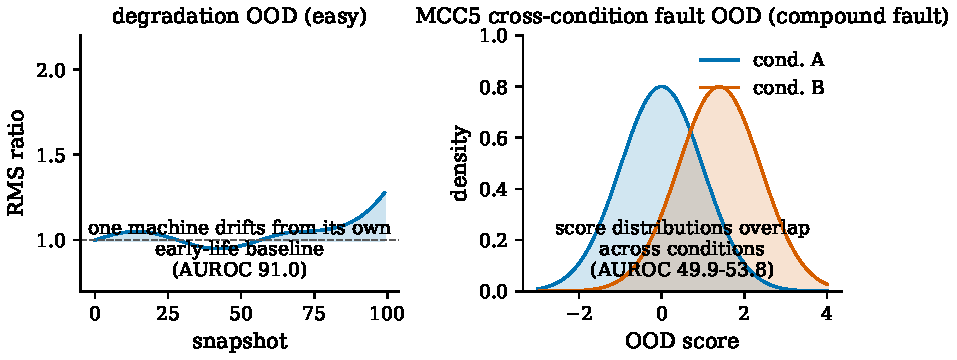
\includegraphics[width=\linewidth]{../figures/fig2_two_problems.pdf}
\caption{Mechanism contrast of the two OOD problems: left, degradation OOD (one machine drifting from its own early-life baseline, AUROC 91.0); right, MCC5 cross-condition fault OOD (score distributions overlap across conditions, AUROC 49.9--53.8).}
\label{fig:twoproblems}
\end{figure}

\begin{table}[!t]
\caption{Degradation-OOD benchmark and cross-condition contrasts: AUROC / FPR95 per method, per dataset, and cross-condition (33 failed bearings, single run; per-method values are per-stream means, per-dataset and macro values are per-bearing means); CASH v1.1 is a causal-anchor OOD scorer (cross-condition baseline).}
\label{tab:ood}
\centering
\begin{tabular}{l l c c}
\toprule
View & Item & AUROC & FPR95\\
\midrule
Method & kNN-5 distance & 96.54 & 10.47\\
Method & Isolation forest & 95.30 & 13.13\\
Method & Mahalanobis & 95.07 & 17.88\\
Method & Centroid distance & 93.00 & 23.94\\
Method & OC-SVM & 92.47 & 27.28\\
Method & RMS ratio & 73.32 & 46.13\\
Method & Reconstruction AE (5$\to$3$\to$5) & 95.62 & 15.56\\
Method & LSTM-AE (unidirectional, 3 seeds) & 95.28 & 14.27\\
Dataset & IMS (4 failed) & 96.89 & 9.75\\
Dataset & XJTU-SY (12) & 96.05 & 13.00\\
Dataset & FEMTO (17) & 86.13 & 33.20\\
Macro & 33 failed bearings & 91.04 & 23.01\\
Cross-cond.\ & CWRU held-condition CASH v1.1 & 96.77 & 5.01\\
Cross-cond.\ & CWRU held-condition Mahalanobis & 93.27 & 11.44\\
Cross-cond.\ & MCC5 held-condition Mahalanobis & 53.79 & 86.01\\
Cross-cond.\ & MCC5 held-condition CASH v1.1 & 49.86 & 91.92\\
\bottomrule
\end{tabular}
\end{table}

Observations from Table~\ref{tab:ood}: (i) kNN, isolation forest, Mahalanobis, centroid, OC-SVM, and the added reconstruction AE (95.6) and LSTM-AE (95.3) all exceed 92.5 AUROC; only the naive RMS ratio (73.3) is markedly low, so ``detecting deviation'' is not hard for mature and deep time-series baselines. (ii) FEMTO is markedly worse than the other two rigs. (iii) The macro FPR95 of 23.01 remains high and, together with the censored contrast (89.32 AUROC), shows the bottleneck is ``separating failure-bound degradation from benign drift at zero false alarms,'' not ``detecting deviation.'' The MLP-AE and LSTM-AE (3-seed per-bearing macro 94.90$\pm$0.21) both fail to beat the best simple baseline (kNN 96.5), further supporting ``degradation OOD is near-solved for simple baselines'' (aggregation note: Table~\ref{tab:ood}'s LSTM-AE 95.28 is a per-stream mean, whereas the 94.90$\pm$0.21 here is the 3-seed per-bearing macro mean---two different aggregation levels, not a contradiction); the macro 91.04 is the per-bearing mean of the six classical baselines and rises to about 91.7 when the AEs are added. The cross-condition rows directly give the corresponding question's second benchmark: CWRU (single bearing fault, speed drift only) held-condition OOD reaches 93.3--96.8, while MCC5 (gear/compound fault, speed+torque drift) is only 49.9--53.8---a gap of about 40 points---so cross-condition difficulty is set by drift type and fault type jointly, not by ``cross-condition is necessarily hard.''

The negative-transfer evidence of cross-condition threshold mismatch is Fig.~\ref{fig:negtransfer}: the same scores give held-condition ID false-positive rates of 2.8/52.7/79.2/27.7\% across the four MCC5 held conditions.

\begin{figure}[!t]
\centering
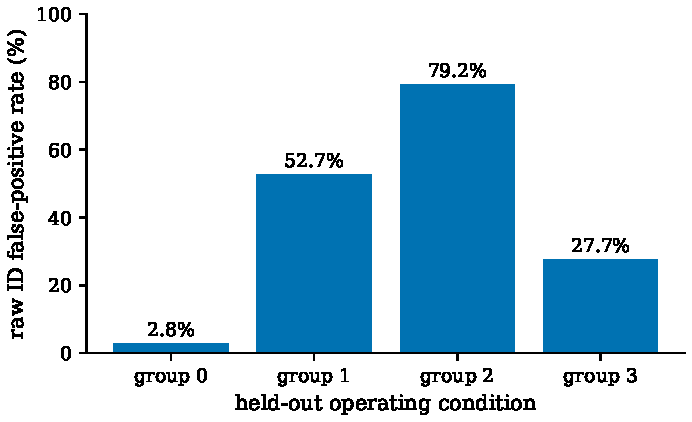
\includegraphics[width=\linewidth]{../figures/fig3_negative_transfer.pdf}
\caption{Negative-transfer evidence: held-condition in-distribution false-positive rates of the raw scores on the MCC5 cross-condition screening, up to 79.2\%.}
\label{fig:negtransfer}
\end{figure}

The four bars in Fig.~\ref{fig:negtransfer} do not sit at one level, meaning the threshold drifts sharply with condition and no single global threshold can suppress the false-positive rate across conditions. This contrasts with degradation OOD's per-machine baseline: the former needs cross-condition calibration, the latter only each machine's early-life baseline. \emph{Not claimed:} ``all degradation detection is easy and all cross-condition detection is hard''---the conclusion is limited to these three datasets and this protocol.

\subsection{Cumulative excess separates failure from drift}\label{sec:rq2}
\emph{Core finding.} The cumulative excess $E_{\mathrm{cum}}$ \eqref{eq:cumexcess} fully separates the four failed from the eight censored IMS bearings (AUROC 100, FPR95 0, exact permutation $p=1/495$, the minimum attainable for a $4$-vs-$8$ full separation), with failed median 0.099 vs.\ censored 0.019 (median ratio $\approx5.2$); the leave-one-bearing AUROC stays 100 (12/12), and the bootstrap 20{,}000-times CI degenerates to $[100,100]$. This result is read as \emph{mechanistic evidence}---it proves the ``persistence'' signal exists---rather than as a performance claim on $n=4$.

Fig.~\ref{fig:faildrift} shows the mechanism on real trajectories: the failed bearing (inner race, test1 B3) and the censored bearing (test1 B1) both cross the $1.2\times$ line many times, so ``exceeded or not'' alone cannot separate them; in the lower panel the failed bearing's rate $R_t$ grows persistently past the threshold $T$ while the censored bearing stays below.

\begin{figure}[!t]
\centering
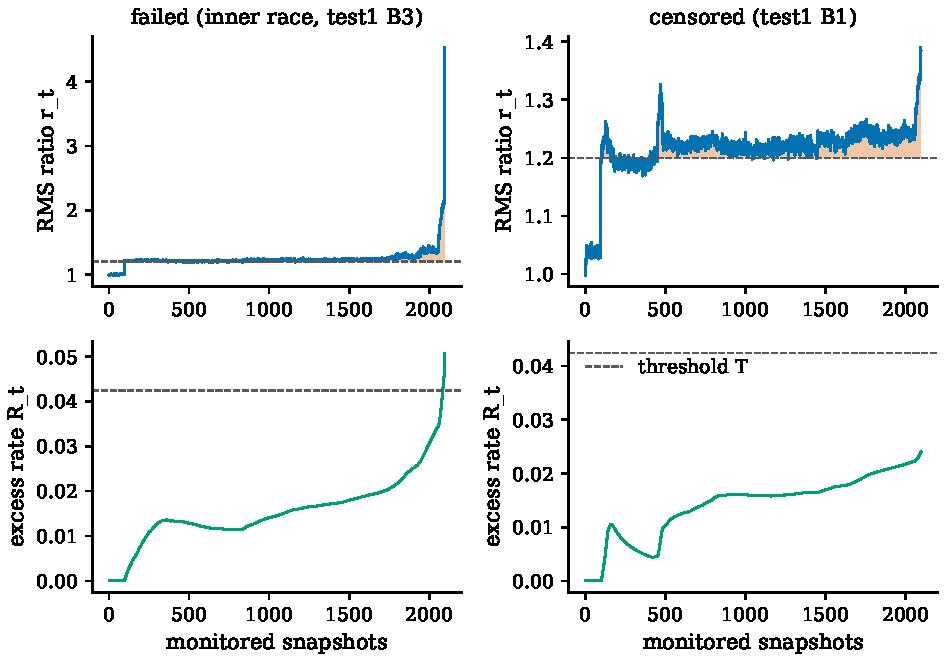
\includegraphics[width=\linewidth]{../figures/fig4_failure_vs_drift.pdf}
\caption{The ``persistence $>$ amplitude'' mechanism on real IMS trajectories: the failed bearing persistently exceeds $1.2\times$ baseline and accumulates excess, while the censored bearing only exceeds occasionally; lower panels show the corresponding excess rate $R_t$ and threshold $T$.}
\label{fig:faildrift}
\end{figure}

\emph{Not claimed:} $n=4$; the significance is real (the $p$-value is already the minimum attainable) but generalizability is unproven, so this is not used as the headline number.

\subsection{Rate-normalized detector and lead time}\label{sec:rq3}
\emph{Core finding.} At the zero-false-alarm operating point ($T=0.0424$) it detects 31/34 (95\% CI 76.3--98.1\%), false alarms 0/8 (95\% CI 0--36.9\%); median lead times are 14.5\%/46.3\%/36.0\% of life (about 23.2 h / 1.1 h / 1.3 h); per-axis 58/66 (87.9\%) vs.\ per-bearing 91.2\%. Cross-dataset heterogeneity is stated explicitly: IMS (4/4) and XJTU-SY (13/13) hit a 100\% ceiling, and FEMTO (14/17 = 82.4\%) is the only genuine cross-rig generalization test. The three FEMTO misses' ``low-amplitude degradation'' is data-supported (Appendix~\ref{app:baselines}): the missed bearings have median max RMS ratio 4.15 and median cumulative excess 62.3, versus 7.82 and 306.5 for the detected bearings---the misses are low-amplitude and low-persistence jointly, not random failures.

Fig.~\ref{fig:opcurve}'s $c$-sweep shows that $c=1.2$ is the ``31/34 detection + 28.8\% median lead time'' trade-off point; larger $c$ (1.55 and 1.8--2.0) reaches 32/34 (94.1\%), but the lead time declines overall as $c$ grows, reaching only 17.5\% at $c=2.0$ (about 11 points lost relative to $c=1.2$), whereas $c=1.55$ loses only about 3 points.

\begin{figure}[!t]
\centering
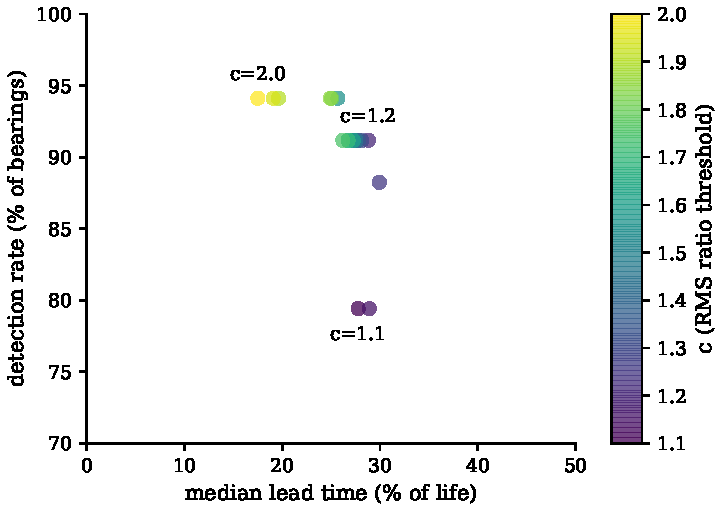
\includegraphics[width=\linewidth]{../figures/fig5_operating_curve.pdf}
\caption{Operating curve over the threshold $c$: every $c$ is re-calibrated to zero false alarms on the censored set, dots are per-bearing detection rate vs.\ median lead time, color encodes $c$.}
\label{fig:opcurve}
\end{figure}

Each $c$ in Fig.~\ref{fig:opcurve} independently re-computes the zero-false-alarm threshold on the censored set (zero false alarms holds by construction), so the curve is non-monotonic and is the true ``detection--lead-time'' trade-off; raising $c$ can at most move detection from 31/34 to 32/34 while pushing lead time from 28.8\% down to 17.5\% (a marginal gain of one bearing at a cost of about 11 points of lead time), so $c=1.2$ is retained; this sweep supports $c=1.2$ independently of the external protocol~\cite{hora_submitted,hora_unpublished}. \emph{Not claimed:} zero false alarms is by construction, not discovered. To turn the ``only 8 IMS censored bearings'' weakness into a measurable number, we add a cross-rig false-alarm proxy (Appendix~\ref{app:baselines}): taking the first 150 snapshots of each XJTU-SY/FEMTO bearing as an early-life pseudo-health segment (these bearings eventually fail but are healthy in the segment), the exceedance rate against $T=0.0424$ is a point estimate of 18.5\% per axis (10 of 54 axes; 95\% CI 9.3--31.4\%; XJTU-SY 30\%, FEMTO 11.8\%) and about 22\% per bearing---an estimate of pseudo-health segments, not a strict upper bound. The threshold therefore transfers across rigs only at a measurable residual cost, which we disclose rather than hide.

\subsection{Comparison with classical and modern baselines}\label{sec:rq4}
\begin{figure}[!t]
\centering
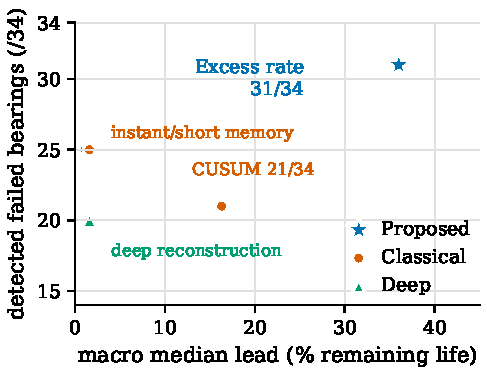
\includegraphics[width=\linewidth]{../figures/fig9_method_tradeoff.pdf}
\caption{Detection--lead-time trade-off under the same causal protocol and zero-false-alarm calibration. The horizontal coordinate is the median of the three per-dataset median lead times. SPRT is omitted because it detects only one failed bearing, and seed-unstable Deep SVDD/RUL-LSTM are omitted because they have no meaningful aggregate lead time. Among the stable baselines shown, the excess-rate detector is Pareto-dominant: it provides both the largest detection count and the longest macro median lead.}
\label{fig:tradeoff}
\end{figure}

\emph{Core finding.} Under the same protocol and zero-false-alarm calibration, excess rate 31/34 $>$ Shewhart 25 $\approx$ EWMA 25 $>$ CUSUM 21 $>$ SPRT 1, and it is well above all four window-level deep reconstruction baselines (MLP-AE, LSTM-AE, Transformer-AE, TranAD, each 20/34) and the supervised RUL-thresholded baseline (median 6/34) (Table~\ref{tab:detectors}; baseline statistics in \eqref{eq:shewhart}--\eqref{eq:sprt} and Appendix~\ref{app:baselines}).

\begin{table}[!t]
\caption{Per-dataset detection count and median lead time of the online detectors under zero-false-alarm calibration (34 failed + 8 censored).}
\label{tab:detectors}
\centering
\begin{tabular}{l c c c c c c}
\toprule
Detector & Det.\ (/34) & IMS & XJTU-SY & FEMTO & Median lead (\%) & Zero-FA thr.\\
\midrule
Excess rate (ours) & 31 & 4/4 & 13/13 & 14/17 & 14.5 / 46.3 / 36.0 & 0.042\\
Shewhart & 25 & 2/4 & 11/13 & 12/17 & 0.7 / 6.8 / 1.1 & 5.69\\
EWMA & 25 & 2/4 & 11/13 & 12/17 & 0.6 / 6.4 / 1.6 & 3.53\\
CUSUM & 21 & 3/4 & 9/13 & 9/17 & 4.4 / 16.3 / 27.3 & 169.5\\
SPRT & 1 & 1/4 & 0/13 & 0/17 & 37.8$^{\ddagger}$ / --- / --- & $1.13\times10^{6}$\\
MLP-AE (window) & 20 & 3/4 & 9/13 & 8/17 & 0.2 / 1.2 / 25.1 & $2.4\times10^{5}$\\
LSTM-AE (unidir.) & 20 & 3/4 & 9/13 & 8/17 & 0.2 / 1.2 / 25.1 & $2.4\times10^{5}$\\
Transformer-AE (causal) & 20 & 3/4 & 9/13 & 8/17 & 0.2 / 1.6 / 25.7 & $2.4\times10^{5}$\\
TranAD (causal) & 20 & 3/4 & 9/13 & 8/17 & 0.2 / 1.6 / 25.7 & $2.4\times10^{5}$\\
Deep SVDD (3-seed median) & 2 & 1/4 & 1/13 & 0/17 & --- & 0.26\\
RUL-LSTM (supervised, 3-seed median) & 6 & 1/4 & 4/13 & 5/17 & --- & 0.13\\
\bottomrule
\end{tabular}
\par\vspace{2pt}
{\footnotesize Zero-false-alarm thresholds are calibrated on the 8 IMS censored bearings; McNemar/Holm significance is in the text. $^{\ddagger}$ SPRT's 37.8\% lead is based on a single sample (IMS 1/4) and carries no statistical meaning; the remaining SPRT lead times are empty. The four reconstruction baselines (MLP-AE/LSTM-AE/Transformer-AE/TranAD) all have a threshold ($\approx2.4\times10^{5}$) dominated by one drifted window of censored bearing test3\_b4; Deep SVDD (1/22/2 across seeds) and RUL-LSTM (theta 0.13 to $-0.03$) are seed-unstable, so their medians are reported.}
\end{table}

Observations: Shewhart and EWMA detect a tolerable 25 but with near-zero lead time (0.6--6.8\%), of no operational value for predictive maintenance; CUSUM and SPRT are nearly or fully destroyed (21/34 and 1/34) by integrating benign drift and the consequently raised zero-false-alarm threshold; SPRT's 1/34 is not an implementation artifact but the inevitable outcome of its misspecified Gaussian null, under which the log-likelihood ratio drifts positively under benign drift (Proposition~1, Appendix~\ref{app:proof}). The four window-level deep reconstruction baselines (MLP-AE/LSTM-AE/Transformer-AE/TranAD) all detect exactly 20/34 with the identical 3/9/8 per-dataset split: their per-window reconstruction error is an \emph{unbounded magnitude quantity} dominated by the window's distance from the healthy training support rather than by learned fault structure, and a drifted window of the censored bearing test3\_b4 (RMS ratio 5.63) raises the zero-false-alarm threshold to about $2.4\times10^{5}$, suppressing detection---the same benign-drift-threshold mechanism as CUSUM/SPRT, but realized through per-window magnitude rather than accumulation. Deep SVDD is unstable when trained on only about 50 healthy windows (1--22/34 across seeds). The supervised RUL-thresholded baseline is trained in-sample on all failed bearings and evaluated on the same bearings---an upper-bound (favorable) treatment for a baseline---yet it remains seed-unstable (median 6/34, best 29/34): it must extrapolate remaining life for the never-failing censored bearings, and that extrapolation swings between positive and negative values across seeds, collapsing the threshold. Paired McNemar exact tests (34 failed bearings): vs.\ CUSUM discordant pairs 10/0 ($p=0.002$, Holm $p=0.006$), vs.\ SPRT 30/0 ($p<0.001$, Holm $p<0.001$) are significant; vs.\ Shewhart/EWMA 6/0 each (raw $p=0.031$, Holm $p=0.063$) is nominally significant but does not survive four-way correction.

\emph{Normalized-accumulator fairness check.} The rate $R_t=S_t/(t-60)$ is, by construction, a zero-drift-compensation, no-reset, time-normalized CUSUM. To rule out ``beating an unbounded strawman,'' we add, under the same protocol, a normalized reset CUSUM ($U_t=\max(0,U_{t-1}+e_t-\delta)$ divided by $t-60$, $\delta\in\{0,0.005,0.01,\hat\mu\}$, with $\hat\mu=0.0153$ the censored mean drift) and a normalized SPRT ($\Lambda_t/(t-60)$): $\delta=0$ reduces to the rate (31/34, a self-check); $\delta=0.005$ gives 31/34; $\delta=0.01$ and $\delta=\hat\mu$ drop to 30/34; normalized SPRT gives only 4/34. Within the normalized-accumulator family, zero drift compensation and no reset is therefore optimal---drift compensation must estimate $\mu$ from only eight censored bearings, and the estimation error lowers sensitivity; normalization cannot repair SPRT's misspecified Gaussian null (Appendix~\ref{app:baselines}).

Fig.~\ref{fig:tradeoff} condenses the deployment-relevant comparison: the excess-rate detector is the only displayed method that combines high detection with substantial lead time. Fig.~\ref{fig:ratecum} visualizes the failure mechanism of unbounded accumulators: on censored bearings the CUSUM/SPRT scores climb monotonically with monitoring duration, and after normalizing each score by its own zero-false-alarm threshold, only the rate crosses the normalized line 1.

\begin{figure}[!t]
\centering
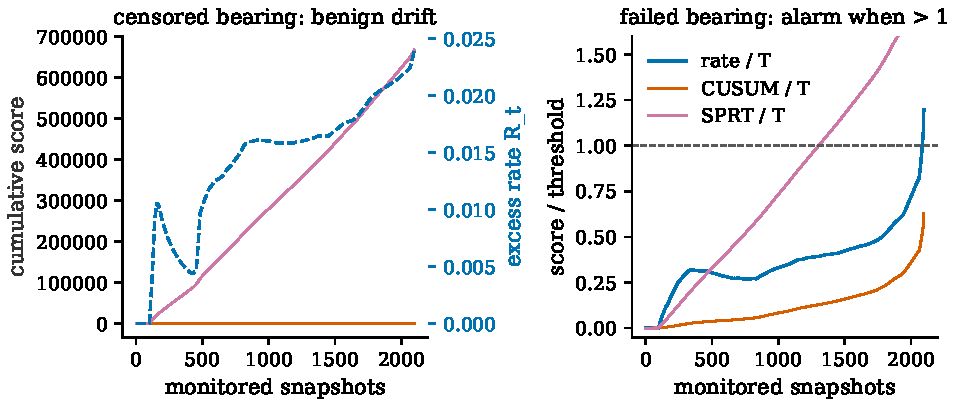
\includegraphics[width=\linewidth]{../figures/fig6_rate_vs_cumulative.pdf}
\caption{What rate normalization buys: (a) benign drift of censored bearings is integrated persistently by CUSUM/SPRT while the rate stays flat; (b) on failed bearings, after normalizing by each score's zero-false-alarm threshold, only the rate crosses 1.}
\label{fig:ratecum}
\end{figure}

\emph{Not claimed:} the detection-count difference between Shewhart/EWMA and the rate does not survive correction; our advantage over them rests mainly on lead time (qualitative) and on the ``unbounded accumulator fails'' result (significant).

\subsection{Ablation and negative results}
\emph{Per-feature ablation (Table~\ref{tab:features}).} Under the same protocol and zero-false-alarm calibration, changing only the scalar feature: RMS 31/34 is best, variance 29/34 second, kurtosis 17/34 worst.

\begin{table}[!t]
\caption{Per-feature ablation (34 failed bearings, same protocol and zero-false-alarm calibration, changing only the scalar feature).}
\label{tab:features}
\centering
\begin{tabular}{l c c c}
\toprule
Feature & Det.\ (/34) & Detection rate (\%) & Median lead (\%) \\
\midrule
RMS (ours) & 31 & 91.2 & 28.8\\
Variance & 29 & 85.3 & 28.3\\
Skewness & 26 & 76.5 & 94.7$^{\dagger}$\\
Peak-to-peak & 24 & 70.6 & 51.6\\
Pearson kurtosis & 17 & 50.0 & 67.9$^{\dagger}$\\
\bottomrule
\multicolumn{4}{l}{\footnotesize $^{\dagger}$ The early-life median of skewness/kurtosis is near zero, so the $1.2\times$ ratio rule is ill-posed for them; their lead-time numbers are not interpreted---the detection rate is the primary ablation output.}
\end{tabular}
\end{table}

\emph{Spectral-feature ablation (negative).} On IMS, envelope kurtosis and fault-frequency envelope ratio give failure-versus-drift AUROC 96.9 / 78.1 and zero-false-alarm detections 2/4 each, not better than RMS (100 / 4/4). \emph{Negative transfer (negative).} On MCC5, requiring $k\ge2$ consecutive exceedances only lowers the ID false-positive rate from about 3\% to about 1\% while delaying E2/E3/E5 alarms by $>730$ windows. \emph{Not claimed:} these negative results do not negate spectral features elsewhere; they only show that for these three rigs the energy (RMS) rise is already a robust early signal.

\emph{Dual-scale activation mechanism probe.} To distinguish historical persistence from recent activation, we additionally compute the causal mean $A_t^{(3)}$ of excess over three monitoring snapshots and independently apply the same 1.01 zero-false-alarm calibration on the IMS censored set. The recent rate alone reaches only 27/34 with 2.94\% median lead, so transient activation cannot replace accumulation; allowing $R_t$ or $A_t^{(3)}$ to cross its calibrated threshold on any axis gives 32/34 and 0/8 false alarms, adding one FEMTO bearing, but the gain disappears when the window increases from three to five snapshots. We use this result as a mechanism probe rather than a headline: historical rate remains the primary signal, and the remaining FEMTO failures still mark the abrupt/low-early-energy boundary.

\emph{Hierarchical cross-axis persistence (exploratory).} The remaining FEMTO misses are not low-amplitude; they show late simultaneous activation on two axes, whereas IMS censored streams contain isolated one-axis transients. Let $A_{k,t}^{(10)}$ denote the ten-snapshot recent excess mean of axis $k$ and $J_t=\mathrm{secondmax}_k A_{k,t}^{(10)}$. By construction, $J_t$ can cross its threshold only when at least two axes corroborate recent activation. The hierarchical rule alarms when any axis has $R_t>T_R$ or $J_t>T_J$. Historical rate, cross-axis rate, and the hierarchy detect 31/34, 32/34, and 34/34, all with 0/8 IMS false alarms; the hierarchy has 28.64\% median lead, and its three additional FEMTO detections occur 0.75\%, 33.46\%, and 1.01\% of life before failure. The hierarchy remains 34/34 for windows 5--100 and margins 1.00--1.20. On 27 early-life pseudo-health bearings, the respective bearing-level false-alarm counts are 6/27, 4/27, and 6/27, so the hierarchy does not worsen the cross-rig proxy. Nevertheless, the three additions have no reversals (exact McNemar $p=0.25$), leave-one-censored-out calibration gives 2/8 held-out false alarms, and only two multi-axis IMS censored bearings calibrate $T_J$. We therefore report this as a mechanism-driven post-hoc extension, not a replacement for the 31/34 headline.

\subsection{Edge cost, robustness, and protocol sensitivity}\label{sec:robustness}
\emph{Core finding.} The detector update takes 0.032 ms/window; the full RMS-extraction-plus-update pipeline takes about 0.038 mJ/window (0.70 W load delta at about 18.3k windows/s), no accelerator (Jetson Orin NX). The two figures are reported separately: 0.032 ms is the pure threshold update, while 0.038 mJ is the energy of the whole overlapping RMS-plus-update pipeline per window; they are not two units of one operation. Robustness (threshold $T=0.0424$ fixed, not re-tuned under perturbation): with 1--10\%-of-baseline zero-mean Gaussian noise on RMS the detection stays 31/34; in the per-bearing per-axis dropout trials (68 runs) the worst is 30/34 and the median 31/34. A causal RMS-feature quantization stress test, using a fixed $[0,8b]$ range set by the already-observed baseline $b$ and no future sample, preserves 31/34 detections and 0/8 false alarms at 8--24 bits; at 8 bits the median lead is 28.46\% versus 28.82\% at full precision. This is a feature-domain result, not a raw-ADC validation. Protocol sensitivity: the detector ordering (excess-rate 31 $>$ Shewhart 25--26 $>$ EWMA 25 $>$ CUSUM 21 $>$ SPRT 1) is invariant to baseline windows 40/50/60; 31/34 is invariant to run-in 5/10/15 and min-monitor 10/30 (min$=$60 gives 30/34). The threshold-margin factor (the $1.01$ in \eqref{eq:threshold}) swept over $\{1.00,1.01,1.05,1.10\}$ always gives 31/34, proving the factor sets only the zero-false-alarm margin, not the detection rate (Appendix~\ref{app:baselines}). The EWMA $\lambda$ swept over $\{0.05,0.1,0.2,0.3,0.5\}$ gives 23/25/25/26/28 (best 28, still below 31); the SPRT alternative mean swept over $\{1.05,1.1,1.2,1.3,1.5\}$ gives 1/1/1/3/6 (best 6, far below 31)---neither sweep changes the Section~\ref{sec:rq4} ranking, ruling out an unfavorable-tuning explanation (Appendix~\ref{app:baselines}).

\subsection{IIoT deployment analysis}\label{sec:deploy}
The rate-normalized detector is an $O(1)$-memory, $O(1)$-time, accelerator-free scalar detector whose deployment form is three-layered: \emph{sensing node} (RMS extraction + per-window rate update) $\to$ \emph{edge gateway} (threshold comparison, latching event, local baseline/threshold) $\to$ \emph{cloud/fleet management} (one-time baseline/threshold batch calibration and alarm aggregation). On the data path, raw waveforms never leave the node and only compact alarm events travel uplink, matching massive-node and narrow-uplink IIoT constraints. This three-layer form is annotated in Fig.~\ref{fig:arch}; energy, bandwidth, and fleet scale are design constraints rather than evaluation appendices. The theoretical properties remain qualitative and do not make individual uplinked alarms statistically trustworthy.

Energy measurement protocol (Jetson Orin NX, 6 cores): jtop/VDD power-rail sampling, 5\,s idle warm-up baseline, 60\,s sustained-loop throughput measurement, five repetitions averaged; the 18{,}266 windows/s throughput corresponds to the full pipeline on XJTU-length windows (32{,}768 samples). Measured idle 5{,}834 mW, load 6{,}533 mW, load delta 698.9 mW, hence 0.0383 mJ per full-pipeline window (698.9 mW $\div$ 18{,}266 windows/s). At the shortest 10\,s snapshot interval the detector's yearly energy is on the order of a hundred joules, and with event-driven reporting it supports long-term deployment under battery or energy-harvesting power. At the fleet level, nodes run independently and the center performs only one-time batch calibration and aggregation, so the system scales horizontally. Risks: the zero-false-alarm threshold depends on healthy censored calibration, and a new rig without healthy-running data cannot guarantee the false-alarm rate (the cross-rig proxy of Section~\ref{sec:rq3} gives about 18\% per axis); very-fast failure and low-amplitude degradation are two known blind spots.

\subsection{Fleet-scale false-alarm budget}
Per-machine zero-false-alarm calibration does not compose across a fleet. Using the cross-rig early-life proxy $q=0.185$ as a modeled per-axis probability (Fig.~\ref{fig:fleet}), a two-axis machine has at least one false event with probability $1-(1-q)^2\approx33.6\%$; 10 machines reach 98.3\%, and 100 dual-axis machines yield 37 expected false events. A bearing-clustered rate $q=0.222$ gives about 22 false events per 100 machines, with bootstrap 95\% CI $[11,67]$. Keeping the fleet-wide probability below 5\% would require $q\approx0.0256\%$, roughly a $720\times$ tightening relative to 18.5\%. These are modeled capacity estimates, not measured fleet alarms; practical control requires empirical calibration, multi-axis confirmation, event aggregation, and hierarchical thresholds.

\begin{figure}[!t]
\centering
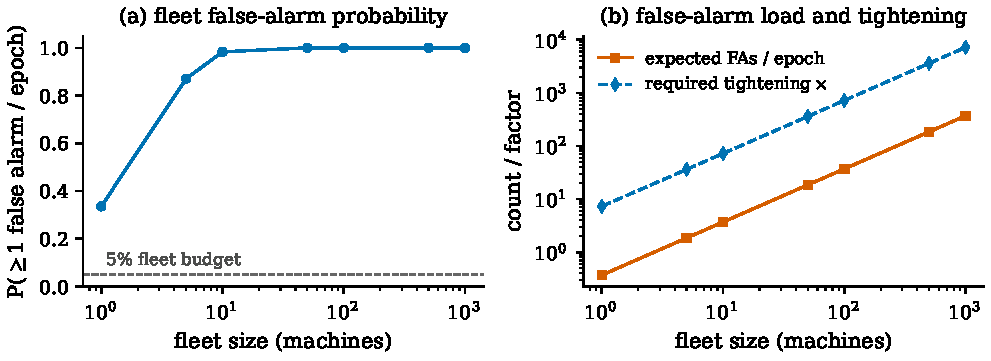
\includegraphics[width=\linewidth]{../figures/fig8_fleet_false_alarm.pdf}
\caption{Fleet-scale false-alarm budget: (a) the fleet-wide ``at least one false alarm per epoch'' probability saturates to one as fleet size grows; (b) expected false alarms per epoch grow linearly with fleet size, and the required per-axis tightening to keep a 5\% fleet budget grows super-linearly (log scale).}
\label{fig:fleet}
\end{figure}

\begin{figure}[!t]
\centering
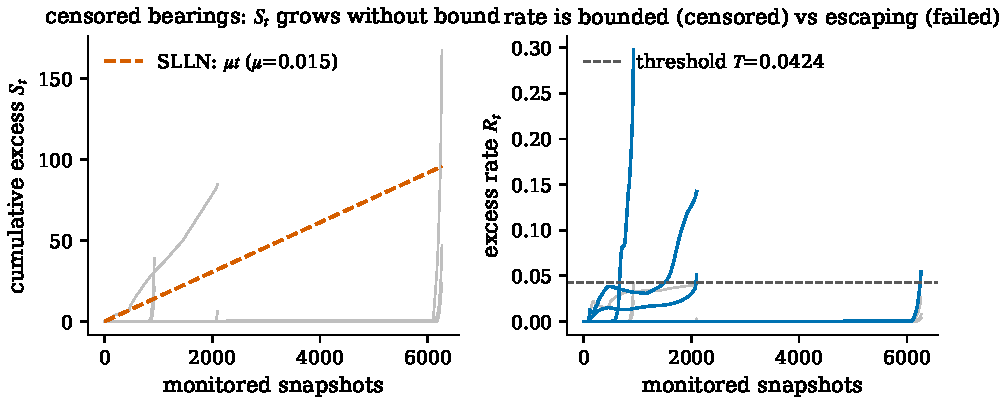
\includegraphics[width=\linewidth]{../figures/fig7_rate_length_invariance.pdf}
\caption{Data-side validation of the rate-normalization mechanism: (a) the cumulative excess $S_t$ of the eight censored bearings grows linearly with monitoring duration, matching the $\mu t$ reference ($\mu=0.0153$, the per-snapshot excess averaged over the censored bearings), so any fixed threshold is eventually crossed; (b) the rate $R_t$ of the same bearings is bounded and converges, and only failed bearings cross the fixed threshold $T=0.0424$.}
\label{fig:theory}
\end{figure}

\subsection{External alarm coverage and operating-condition boundary}
On LDM\_UPB, the frozen protocol triggers all 11 protocol-qualified experiments without changing threshold, window, or cross-axis rule; historical-rule coverage is 11/11. The median monitoring-segment lead is 95.9\%, but LDM\_UPB has no preregistered fault onset, so this is not a remaining-life fraction or proof of early fault detection. Eight of 11 experiments trigger at the earliest permitted monitoring point. Figure~\ref{fig:condition} shows that B01 triggers when dynamic load changes by 35.5\% and speed by 27.5\%, whereas B11 triggers later under a more stable condition. Thus, a fixed RMS baseline can mistake an operating-condition response for persistent excess. A ridge-residual probe delays five of eight early alarms and reduces median lead to 63.2\%, but it is post hoc and does not change the main method.

\begin{figure}[!t]
\centering
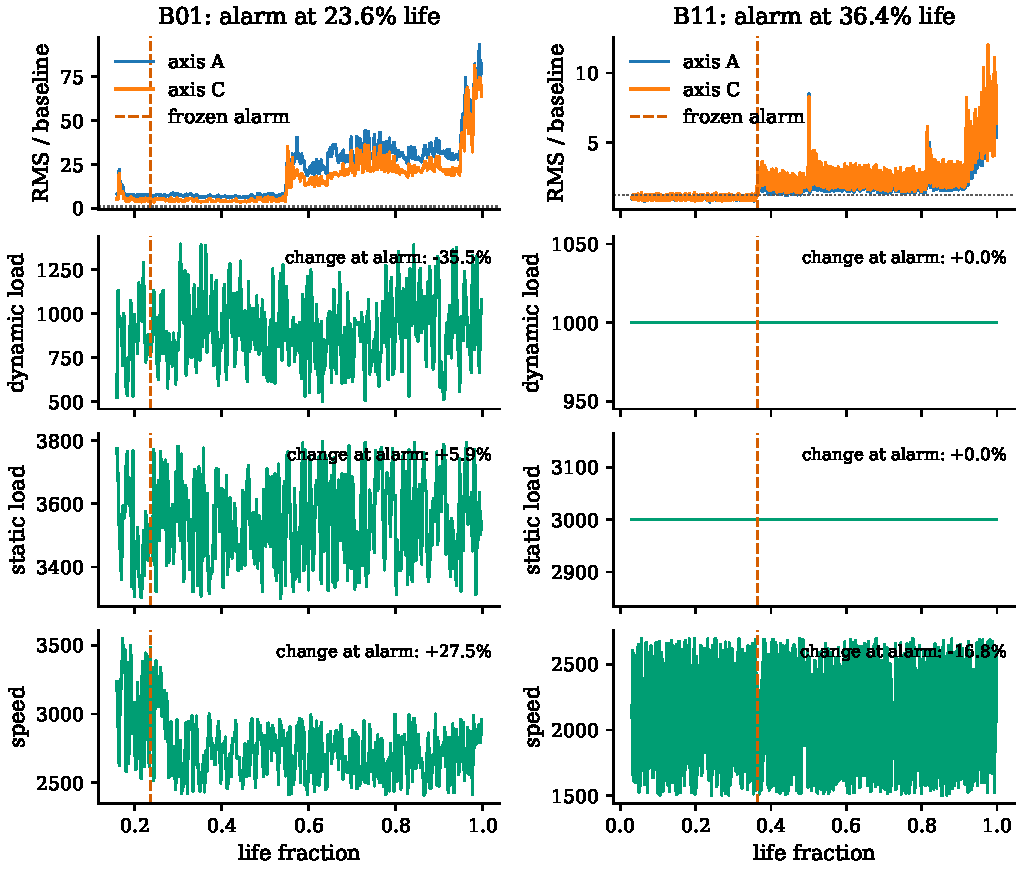
\includegraphics[width=\linewidth]{../figures/fig10_ldm_upb_condition_sensitivity.pdf}
\caption{RMS and operating-condition changes in the external LDM\_UPB replication.}
\label{fig:condition}
\end{figure}

\subsection{Healthy evidence and system-level stress tests}\label{sec:risk}
\subsubsection{Five-tier healthy-evidence ladder}
Table~\ref{tab:healthy-evidence} expands a single 0/8 calibration result into real calibration, real held-out data, steady-state normal records, cross-rig early-life proxies, and a virtual multi-rig mechanism stress test. The tiers do not establish a universal false-alarm rate; they expose its uncertainty.

\begin{table}[!t]
\centering
\caption{Five-tier healthy-evidence ladder.}
\label{tab:healthy-evidence}
\begin{tabular}{clrl}
\toprule
Tier & Evidence source & Alarms/sample & Boundary \\
\midrule
1 & IMS in-sample censored & 0/8 & Calibration only \\
2 & IMS leave-one-experiment & 1/8 & Small-sample sensitivity \\
3 & CWRU steady normal & 0/3 & Not censored or multi-rig \\
4 & XJTU/FEMTO pseudo-health & 6/27 & Not full healthy life \\
5 & Virtual eight-rig cohort & 2/24 & Mechanism stress only \\
\bottomrule
\end{tabular}
\end{table}

\subsubsection{D1-causal-three}
Public D1 uses a 1.2 threshold, three consecutive crossings, and persistence to the endpoint. It detects 33/34 in this cohort but produces reference-zone episodes in 2/8 censored bearings. D1-causal-three removes endpoint persistence and latches at the first third consecutive crossing: it detects 34/34 failures but alarms on all 8/8 censored bearings. Therefore D1's apparent advantage depends on future endpoint confirmation rather than a stronger online event rule.

\subsubsection{Shewhart/EWMA interpretation}
Against Shewhart and EWMA, RNED has six favorable and zero unfavorable discordant pairs. The raw exact McNemar $p$ is 0.03125, but Holm correction over four comparisons gives 0.0625. A Beta$(7,1)$ posterior has mean 0.875 and equal-tailed 95\% interval 0.590--0.996; it is directional auxiliary evidence, not a replacement for the frequentist test.

\subsubsection{Virtual multi-node IoT network}
The deterministic network has 100 dual-axis machines, 200 axes, and 5{,}000 cycles. Event probability is 0.01 per axis, inter-axis correlation is 0.2, and uplink latency is lognormal with median 30.0~ms. Data and ACK packets are independently lost; event IDs are deduplicated and unreachable events are censored at 1{,}000~ms. Without loss, event traffic saves 98.043\% bytes. Under 10\% loss, one retry gives 98.999\% delivery and 92.61~ms p95 completion; three retries give 100\% and 84.70~ms but 9.643\% duplicates.

\subsubsection{From one machine to fleet capacity}
If each machine has false-event probability $q$, $F$ machines produce at least one false event with probability $1-(1-q)^F$. For $q=1\%$, 100 machines reach 63.4\%; keeping the probability below 5\% requires $q\approx0.0513\%$. Eight calibration trajectories cannot identify such a tail quantile reliably, motivating conservative upper confidence quantiles and secondary confirmation.

\section{Discussion}\label{sec:discussion}
\subsection{Answers to the core questions}
First, full-life time-averaged excess completely separates IMS failure from censored bearings, while instantaneous exceedances overlap; fixed-window separation weakens. The signal combines exceedance frequency, positive magnitude, and late degradation information, so it is not a universal physical law. Second, the online rate detects 31/34 with 0/8 in-sample alarms, 1/8 held-out alarms, and 14.5--46.3\% median leads under the frozen protocol. Third, compared with the single-sample RMS ratio and unnormalized CUSUM, discordant pairs are 6/0 and 10/0, but these are post hoc multiple comparisons. D1's 33/34 depends on endpoint semantics; deep and RUL baselines are weaker under the same calibration but do not rule out other models. Fourth, measured edge cost and deterministic network accounting satisfy the tested environment; the absence of multiple boards, real ADCs, real networks, and field data prevents a complete IIoT-system claim.

\subsection{Mechanism interpretation and evidence boundary}
Instantaneous exceedance alone cannot separate failure from drift. Full-life excess separates the small IMS cohort, but fixed common-window separation is not significant; occupation and positive magnitude alone do not explain the result. RMS is robust relative to other scalar features in this protocol, yet it remains condition-sensitive. The physical interpretation is an energy proxy for cumulative degradation, not a fitted damage model.

\subsection{Relation to prior work}
BA-RNED does not replace sequential testing, deep anomaly detection, diagnosis, or RUL regression. It supplies a causal, low-state first-event rule and an explicit communication/fleet budget layer that can trigger a higher-capacity diagnostic model or human confirmation.

\subsection{Failure conditions and negative results}
The main misses are low-amplitude, low-persistence FEMTO bearings. Cross-rig pseudo-health and the virtual cohort reveal false-alarm risk. The hierarchical rule can reach 34/34 and 0/8 in-sample but raises held-out alarms to 2/8 and lacks independent validation. These results bound the claim rather than invalidate the method.

\subsection{Engineering significance}
One accumulator, one counter, sub-millisecond updates, compact events, and explicit retry/deduplication make the rule suitable as a first-layer trigger. Fleet thresholds require calibration capacity planning; merely raising the node threshold first sacrifices low-energy failures.

\subsection{Limitations and future work}
The evidence lacks an independent real multi-rig healthy-censored cohort, real wireless broker experiments, multi-board energy measurements, and maintenance-value validation. Future work should collect preregistered external cohorts, test MQTT/CoAP and security stacks, incorporate condition-aware calibration, and connect events to work orders.

\section{Conclusion}\label{sec:conclusion}
BA-RNED unifies causal node detection, gateway event transport, and fleet false-event budgeting. RNED detects 31/34 failed bearings with 14.5\%, 46.3\%, and 36.0\% median leads on IMS, XJTU-SY, and FEMTO; in-sample and held-out censored alarms are 0/8 and 1/8, while the virtual eight-rig cohort gives 2/24 and rules out an inherent zero-alarm claim. D1-causal-three shows that D1's apparent 33/34 advantage depends on endpoint confirmation. The virtual 100-machine network saves 97.6--98.0\% bytes and reaches 100\% delivery with three retries at the cost of 9.643\% duplicates. BA-RNED is therefore a low-state, reproducible, boundary-aware IIoT event baseline, not a theoretical zero-false-alarm guarantee or a complete physical-network deployment claim.

\appendix
\section{Proofs of Propositions 1--2}\label{app:proof}
Let $n=t-60$, reindex the excess sequence as $e_1,\dots,e_n$, $S_n=\sum_{i=1}^{n}e_i$, and $R_n=S_n/n$.

\textbf{Proof of Proposition 1.} If $\{e_i\}$ is strictly stationary and ergodic with $\mathbb{E}[e_1]=\mu>0$, Birkhoff's ergodic theorem gives $S_n/n\to\mu$ almost surely. Hence $S_n\to\infty$ and every finite fixed threshold is eventually crossed. For CUSUM, drift compensation $\delta<\mu$ leaves a positive-mean increment. For SPRT under a misspecified healthy null, the expected pre-reset log-likelihood increment can be positive; the reflected process is then a positive-drift random walk and is unbounded. Thus, a fixed zero-false-alarm threshold for an unbounded accumulator must grow with duration, which can miss late real failures. Table~\ref{tab:detectors} reports the corresponding empirical failures (CUSUM 21/34 and SPRT 1/34).

\textbf{Proof of Proposition 2.} Stationarity and linearity give $\mathbb{E}[R_n]=(1/n)\sum_i\mathbb{E}[e_i]=\mu$, independent of monitoring duration. For $a>0$, $R_n(ae)=aR_n(e)$, yielding first-order scale equivariance. These are qualitative design properties only; they require the stated mean assumption and do not provide a numeric finite-population false-alarm bound.

\section{Added contrast experiments and baseline definitions}\label{app:baselines}
\subsection*{CASH v1.1 contrast baseline}
CASH v1.1 (causal-anchor sparse-graph scorer) is a cross-condition OOD baseline from our companion work, used only as a contrast in Table~\ref{tab:ood} and not part of the online-warning contribution. Definition: 64-dimensional time/spectrum/envelope features per window; sparse causal-anchor graphs built from class anchors and class$\times$condition anchors of the training set (top-$k$ incoming edges, no test--test edges); score $S_{\mathrm{CASH}}=\max(S_{\mathrm{energy}},S_{\mathrm{anchor}},S_{\mathrm{support}})$ with $S_{\mathrm{energy}}$ the energy residual, $S_{\mathrm{anchor}}$ the anchor-reconstruction residual, and $S_{\mathrm{support}}$ the ID-support residual; higher is more OOD. CWRU and MCC5 both use held-condition protocols, training on known ID conditions and evaluating AUROC/FPR95 on the held condition.

\subsection*{Window-level deep online baseline configuration (Section~\ref{sec:rq4})}
All deep baselines share the frozen protocol: per bearing--axis stream, train only on snapshots 11--60, score causally window by window from snapshot 61, aggregate per bearing as the max over axes, and calibrate the zero-false-alarm threshold on the 8 IMS censored bearings by \eqref{eq:threshold}; each is run over three seeds (0/1/2). The MLP autoencoder is $5\to3\to5$ (tanh hidden), Adam, lr$=$0.01, 300 epochs, scored by per-window reconstruction MSE; the LSTM autoencoder is a unidirectional encoder--decoder (hidden 16), Adam, lr$=$0.005, 300 epochs, scored by per-timestep MSE; the causal Transformer autoencoder is a causally-masked Transformer encoder with a learned start token ($d{=}16$, 2 heads, 1 layer), Adam, lr$=$0.005, 200 epochs, scored by per-timestep MSE; TranAD is a two-encoder (focus/backbone) plus decoder trained with 100 reconstruction epochs then 100 adversarial epochs (backbone frozen, focus amplifying reconstruction error), scored by its phase-1 error; Deep SVDD uses a $5\to16\to8\to4$ encoder with the center fixed as the mean of the initial encodings, Adam, lr$=$0.005, 500 epochs, scored by squared distance to the center. The four reconstruction baselines (MLP-AE/LSTM-AE/Transformer-AE/TranAD) all converge to the identical 3/9/8 per-dataset split and a $\approx2.4\times10^{5}$ threshold: their reconstruction error is dominated by the window's distance from the healthy training support, independent of architecture. Deep SVDD is highly seed-sensitive (total detection 1/22/2), so Table~\ref{tab:detectors} reports its median with an instability note.

\subsection*{Supervised RUL-thresholded baseline (Section~\ref{sec:rq4})}
A unidirectional LSTM (hidden 16) regresses the remaining-life fraction $(N-t)/(N-60)$ on all failed bearing--axis streams (monitoring region only), Adam, lr$=$0.005, 8 passes over the dataset. The model is trained in-sample on all failed bearings and evaluated on the same bearings---an upper-bound (favorable) treatment for a baseline. The alarm rule is ``predicted remaining-life fraction $<$ threshold,'' with the threshold set to the minimum predicted value over the censored bearings (zero false alarms by construction), over three seeds. Even under this favorable setting the baseline is seed-unstable (total detection 29/5/6, median 6/34): the model must extrapolate remaining life for the never-failing censored bearings, and that extrapolation swings between positive and negative values across seeds, collapsing the threshold.

\subsection*{Fleet-scale false-alarm budget (Section~\ref{sec:deploy})}
Let a fleet contain $F$ machines with $K$ axes each, and let $q$ be the fixed marginal false-event probability. The independent-axis model gives $P_{\mathrm{fleet}}=1-(1-q)^{FK}$. With the cross-rig early-life proxy $q=0.185$, the model exposes the noncomposition of per-node zero alarms but is not an estimated real-fleet false-alarm rate or a distribution-free upper bound.

\subsection*{Normalized accumulators and robustness checks (Sections~\ref{sec:rq3}/\ref{sec:rq4}/\ref{sec:deploy})}
Normalized accumulators: $U_t=\max(0,U_{t-1}+e_t-\delta)$ divided by $t-60$, with $\delta\in\{0,0.005,0.01,\hat\mu\}$, gives 31/31/30/30; normalized SPRT $\Lambda_t/(t-60)$ gives 4/34. FEMTO misses: missed bearings have median max RMS ratio 4.15 and cumulative excess 62.3, versus 7.82 and 306.5 for detected bearings. Fleet bootstrap: only 2 of 54 pseudo-health axes belong to bearings with mixed-axis alarms, the bearing-level rate is $q=0.222$, and the bootstrap 95\% CI for a 100-machine fleet is $[11,67]$ false alarms per epoch. Mixing decay: censored excess autocorrelation at lags 1/5/20 is 0.92/0.90/0.80 with fitted power-law exponent $a\approx0.18$. Causal RMS quantization maps each monitoring feature to an 8-bit-or-finer uniform grid on $[0,8b]$ using only the already-observed baseline $b$, while keeping $T$ unchanged; all tested 8--24-bit settings retain 31/34 and 0/8. Scripts \texttt{run\_to\_failure\_normalized\_accumulators.py}, \texttt{run\_to\_failure\_robustness\_checks.py}, and \texttt{run\_to\_failure\_deployment\_value\_experiments.py}, with results under \texttt{results/}.

\subsection*{Dual-scale activation mechanism probe (Sections~\ref{sec:results} and \ref{sec:discussion})}
For each axis stream define $A_t^{(w)}=w^{-1}\sum_{j=t-w+1}^{t}e_j$ (using an expanding mean before $w$ observations), with $w=3$ as the primary probe and $w\in\{2,3,5,10,20\}$ as sensitivity. $R_t$ and $A_t^{(w)}$ receive independent thresholds equal to 1.01 times their full-trajectory maxima on the eight IMS censored bearings; a bearing alarms when either statistic crosses its threshold on any axis. With $w=3$, historical rate gives 31/34 (28.82\% median lead), recent rate 27/34 (2.94\%), and dual-scale activation 32/34 (28.64\%), all with 0/8 IMS false alarms. Dual activation adds FEMTO Bearing2\_4 but still misses Bearing1\_5 and Bearing1\_6. Across windows 2/3/5/10/20, dual detection is 32/32/31/31/31, so the one-bearing gain is not promoted to a headline result. Script: \texttt{run\_to\_failure\_rate\_acceleration.py}; result file: \texttt{results\_run\_to\_failure\_rate\_acceleration.json}.

\subsection*{Hierarchical cross-axis persistence (Sections~\ref{sec:results} and \ref{sec:discussion})}
Let $A_{k,t}^{(10)}$ be the ten-snapshot recent excess mean of axis $k$ and $J_t=\mathrm{secondmax}_k A_{k,t}^{(10)}$. Calibrate $T_R$ and $T_J$ independently as 1.01 times their full-trajectory maxima over the IMS censored streams (for $J_t$, only multi-axis streams enter). A bearing alarms when any axis has $R_t>T_R$ or $J_t>T_J$. Historical rate, cross-axis rate, and the hierarchy detect 31/34, 32/34, and 34/34, all with 0/8 IMS false alarms; the hierarchy has 28.64\% median lead, with 20 historical-layer and 14 cross-axis-layer alarms. Detection remains 34/34 for windows $\{5,8,10,15,20,30,50,80,100\}$ and margins $\{1.00,1.01,1.03,1.05,1.10,1.20\}$. On 27 early-life pseudo-health bearings, the three rules give 6/27, 4/27, and 6/27 bearing-level false alarms. The exact McNemar test for 31 versus 34 with three one-way discordant pairs gives two-sided $p=0.25$; leave-one-censored-out calibration gives 2/8 held-out false alarms. Script: \texttt{run\_to\_failure\_cross\_axis\_persistence.py}; result file: \texttt{results\_run\_to\_failure\_cross\_axis\_persistence.json}.

\subsection*{New experiment scripts}
The experiments correspond to \texttt{run\_to\_failure\_modern\_baselines.py}, \texttt{run\_to\_failure\_transformer\_baselines.py}, \texttt{run\_to\_failure\_rul\_baseline.py}, \texttt{run\_to\_failure\_fleet\_fa\_budget.py}, \texttt{run\_to\_failure\_ewma\_sprt\_sweep.py}, \texttt{run\_to\_failure\_threshold\_epsilon\_sweep.py}, \texttt{run\_to\_failure\_cross\_dataset\_fa\_proxy.py}, \texttt{run\_to\_failure\_rate\_acceleration.py}, \texttt{run\_to\_failure\_cross\_axis\_persistence.py}, and \texttt{run\_to\_failure\_deployment\_value\_experiments.py} in the \texttt{experiments/} directory, with results written to same-named JSON files under \texttt{results/}.

\subsection*{Parameter sweeps (Section~\ref{sec:robustness})}
The threshold-margin factor (the $1.01$ in \eqref{eq:threshold}) swept over $\{1.00,1.01,1.05,1.10\}$ always gives 31/34. The EWMA smoothing $\lambda$ swept over $\{0.05,0.1,0.2,0.3,0.5\}$ gives total detection 23/25/25/26/28. The SPRT alternative mean $\mu_1$ swept over $\{1.05,1.1,1.2,1.3,1.5\}$ gives 1/1/1/3/6. All are reported under the same zero-false-alarm calibration; the ranking is parameter-robust.

\subsection*{Cross-rig false-alarm proxy (Section~\ref{sec:rq3})}
Take the first 150 snapshots of each XJTU-SY (10 bearings, 20 axes) and FEMTO (17 bearings, 34 axes) bearing as an early-life pseudo-health segment (these bearings eventually fail but are healthy in the segment), and evaluate the exceedance rate against $T=0.0424$: XJTU-SY 30.0\%, FEMTO 11.8\%, overall 18.5\% per axis (10 of 54 axes alarm; 95\% CI 9.3--31.4\%) and about 22\% per bearing. The proxy is not a true healthy-bearing sample and serves only as a point estimate of residual false alarms, not a strict upper bound, for threshold transfer.

\section*{Declarations}
\textbf{Data availability.} The primary experiment uses public IMS~\cite{lee2007}, XJTU-SY~\cite{wang2020}, and FEMTO/PRONOSTIA~\cite{nectoux2012}; task-boundary analyses additionally use CWRU~\cite{smith2015}, MCC5~\cite{mcc5dataset}, LDM\_UPB~\cite{javanmardi2024,aimiyekagbon2024}, DLR needle-bearing data~\cite{seferli2026}, and Siemens SCADA~\cite{siemens2026}. Raw public data are not redistributed.

\textbf{Author contributions.} Zhiguo Xiao: conceptualization, methodology, software, formal analysis, writing---original draft, review, and editing. Yujing Guo, Yanqi Shao, Guangteng Chen, Dingbo Hou, Yuanyuan Liu, Xinyao Cao: data curation, investigation, visualization, review, and editing. Junli Liu: supervision and funding acquisition.

\textbf{Conflict of interest.} The authors declare no conflict of interest.

\textbf{Funding.} Jilin Provincial Scientific and Technological Development Program (20260102278JC); 2023 Postgraduate Education and Teaching Reform Research Project of Jilin Province (JJKH20230100YJG); Scientific Research Project of Jilin Provincial Department of Education (JKH20262389CY).

\textbf{AI use disclosure.} AI tools assisted language editing and translation. The authors produced and verified all technical content, derivations, experiments, and conclusions and take full responsibility for the manuscript.

\bibliographystyle{IEEEtran}
\bibliography{references_v20}

\end{document}
